\caulc
\begin{ex}%[2D4N1-3]%[TDMZZ16]%[Bồ Văn Hậu]
	Nguyên hàm của hàm số $f(x)=\sin x$ là
	\choice
	{$\cos x+C$}
	{$\dfrac{1}{2}\sin^2 x+C$}
	{\True $-\cos x+C$}
	{$\tan x+C$}
	\loigiai{Ta có $\displaystyle\int \sin x \mathrm{\,d}x=-\cos x+C$.}
\end{ex}

\begin{ex}%[2D4H3-3]%[TDMZZ16]%[Bồ Văn Hậu]
	Trong mặt phẳng $Oxy$, cho hình phẳng $(H)$ giới hạn bởi đồ thị hàm số $y=x^2-4x+3$ và trục hoành $Ox$. Hãy tính thể tích khối tròn xoay thu được khi cho $(H)$ quay quanh trục $Ox$.
	\choice
	{$\dfrac{16}{15}$}
	{\True $\dfrac{16\pi}{15}$}
	{$\dfrac{4\pi}{3}$}
	{$\dfrac{4}{3}$}
	\loigiai{Phương trình hoành độ giao điểm của đồ thị hàm số $y=x^2-4x+3$ và trục hoành là
		\[x^2-4x+3=0 \Leftrightarrow \hoac{&x=1\\&x=3.}\]
		Thể tích khối tròn xoay thu được khi cho $(H)$ quay quanh trục $Ox$ là
		\[V=\pi \displaystyle\int\limits_1^3 \left(x^2-4x+3\right)^2 \mathrm{\,d}x=\dfrac{16\pi}{15}.\]}
\end{ex}

\begin{ex}%[2D3H1-4]%[TDMZZ16]%[Bồ Văn Hậu]
	Cho một mẫu số liệu ghép nhóm $M$ có độ dài các nhóm bằng nhau và có nhóm thứ nhất là $[1;3)$ và nhóm cuối cùng là $[7;9]$. Biết các mẫu số liệu này là các giá trị của $10$ số hạng đầu của dãy số $(u_n)$ với $u_n=\dfrac{11n+3}{n+4}$. Tần số của nhóm thứ $3$ bằng
	\choice
	{\True $4$}
	{$1$}
	{$3$}
	{$3$}
	\loigiai{Mẫu số liệu ghép nhóm $M$ có độ dài các nhóm bằng nhau nên các nhóm gồm $[1;3)$, $[3;5)$, $[5;7)$, $[7;9]$. Do đó nhóm thứ $3$ là $[5;7)$.\\
		Ta có $10$ số hạng đầu của dãy số $(u_n)$ lần lượt là
		\[u_1=\dfrac{14}{5}; u_2=\dfrac{25}{6}; u_3=\dfrac{36}{7}; u_4=\dfrac{47}{8}; u_5=\dfrac{58}{9}; u_6=\dfrac{69}{10}; u_7=\dfrac{80}{11}; u_8=\dfrac{91}{12}; u_9=\dfrac{102}{13}; u_{10}=\dfrac{113}{14}.\]
		Suy ra $1<u_1<3$; $3<u_2<5$; $5<u_3<u_4<u_5<u_6<7$ và $7<u_7<u_8<u_9<u_{10}<9$.\\
		Bảng tần số ghép nhóm như sau
		\begin{center}
			\begin{tabular}{|c|c|c|c|c|}
				\hline
				Nhóm&$[1;3)$ &$[3;5)$ &$[5;7)$ &$[7;9]$\\
				\hline
				Tần số&$1$ &$1$ &$4$ &$4$ \\
				\hline
			\end{tabular}
		\end{center}
		Vậy tần số của nhóm thứ $3$ bằng $4$.}
\end{ex}

\begin{ex}%[2H5N1-3]%[TDMZZ16]%[Bồ Văn Hậu]
	Trong không gian $Oxyz$, phương trình tổng quát của một mặt phẳng đi qua điểm $A(2;1;1)$ và có một vectơ pháp tuyến $\overrightarrow{n}=(3;-1;2)$ là
	\choice
	{$3x-y+2z-9=0$}
	{$2x+y+z-7=0$}
	{$2x+y+z-9=0$}
	{\True $3x-y+2z-7=0$}
	\loigiai{Phương trình mặt phẳng đi qua điểm $A(2;1;1)$ và nhận $\overrightarrow{n}=(3;-1;2)$ làm vectơ pháp tuyến là
		\[3(x-2)-1(y-1)+2(z-1)=0 \Leftrightarrow 3x-y+2z-7=0.\]}
\end{ex}

\begin{ex}%[2D1N4-1]%[TDMZZ16]%[Bồ Văn Hậu]
	Tiệm cận đứng của đồ thị hàm số $y=\dfrac{x+3}{x-2}$ là
	\choice
	{$x=1$}
	{\True $x=2$}
	{$y=2$}
	{$y=1$}
	\loigiai{Ta có $\displaystyle\lim\limits_{x \to 2^+} \dfrac{x+3}{x-2}=+\infty$; $\displaystyle\lim\limits_{x \to 2^-} \dfrac{x+3}{x-2}=-\infty$ nên đường thẳng $x=2$ là tiệm cận đứng của đồ thị hàm số $y=\dfrac{x+3}{x-2}$.}
\end{ex}

\begin{ex}%[1D6H4-3]%[TDMZZ16]%[Bồ Văn Hậu]
	Tập nghiệm của bất phương trình $\log(x-9)<1$ là
	\choice
	{$(-\infty;19)$}
	{$(19;+\infty)$}
	{\True $(9;19)$}
	{$(0;+\infty)$}
	\loigiai{Điều kiện xác định là $x-9>0 \Leftrightarrow x>9$.\\
		Khi đó $\log(x-9)<1\Leftrightarrow x-9<10 \Leftrightarrow x<19$.\\
		Kết hợp điều kiện $x>9$ ta được $9<x<19$.\\
		Vậy tập nghiệm của bất phương trình là $S=(9;19)$.}
\end{ex}

\begin{ex}%[2H5N2-2]%[TDMZZ16]%[Bồ Văn Hậu]
	Trong không gian $Oxyz$, cho đường thẳng $d \colon \dfrac{x-2}{3}=\dfrac{y-1}{-2}=\dfrac{z}{2}$. Vectơ nào sau đây là một vectơ chỉ phương của $d$?
	\choice
	{\True $\overrightarrow{u}_1=(3;-2;2)$}
	{$\overrightarrow{u}_2=(2;1;0)$}
	{$\overrightarrow{u}_3=(3;2;-2)$}
	{$\overrightarrow{u}_4=(1;3;-2)$}
	\loigiai{Từ phương trình chính tắc của đường thẳng $d \colon \dfrac{x-2}{3}=\dfrac{y-1}{-2}=\dfrac{z}{2}$, suy ra một vectơ chỉ phương của $d$ là $\overrightarrow{u}_1=(3;-2;2)$.}
\end{ex}

\begin{ex}%[1D6N4-2]%[TDMZZ16]%[Bồ Văn Hậu]
	Nghiệm của phương trình $8^x=32$ là
	\choice
	{\True $x=\dfrac{5}{3}$}
	{$x=\dfrac{3}{5}$}
	{$x=5$}
	{$x=3$}
	\loigiai{Ta có $8^x=32 \Leftrightarrow x=\log_8 {32}=\dfrac{5}{3}$.\\
		Vậy nghiệm của phương trình đã cho là $x=\dfrac{5}{3}$.
	}
\end{ex}

\begin{ex}%[1H8H2-3]%[TDMZZ16]%[Bồ Văn Hậu]
	\immini[thm]{Cho hình chóp đều $S. ABCD$ có tâm của đáy là điểm $O$. Hỏi phát biểu nào dưới đây là \textbf{sai}?
		\choice
		{$SO \perp AD$}
		{$AC \perp BD$}
		{$AC \perp SD$}
		{\True $CD \perp SB$}}{\begin{tikzpicture}[scale=0.7, font=\footnotesize, line join=round, line cap=round, >=stealth, declare function={bc=4; ba=2; h=4; gocB=30;}]
			\path
			(0,0) coordinate (B)
			(gocB:ba) coordinate (A)
			(bc,0) coordinate (C)
			($(C)-(B)+(A)$) coordinate (D)
			($(A)!0.5!(C)$) coordinate (O)
			($(O)+(90:h)$) coordinate (S);
			\draw (B)--(C)--(D)--(S)--cycle (S)--(C);
			\draw[dashed] (C)--(A)--(D)--(B) (O)--(S)--(A)--(B);
			\foreach \diem/\goc in {A/160, B/-135, C/-45, D/20, S/90, O/-90}
			\fill[black] (\diem) circle (1.2pt) ++(\goc:0.3) node{$\diem$};
	\end{tikzpicture}}
	\loigiai{Ta có $S. ABCD$ là hình chóp đều có tâm đáy là $O$ nên $SO \perp (ABCD)$ và $ABCD$ là hình vuông. Suy ra $SO \perp AD$ và $AC \perp BD$.\\
		Mà $AC \perp BD$ và $AC \perp SO$ nên $AC \perp (SBD)$ hay $AC \perp SD$.\\
		Vậy phát biểu sai là $CD \perp SB$.
	}
\end{ex}

\begin{ex}%[1D2H3-4]%[TDMZZ16]%[Bồ Văn Hậu]
	Cho cấp số nhân $\left(u_n\right)$ có $u_1=1$; $u_2=2$. Số hạng thứ $6$ của cấp số nhân này bằng
	\choice
	{$64$}
	{$11$}
	{\True $32$}
	{$16$}
	\loigiai{Công bội của cấp số nhân là $q=\dfrac{u_2}{u_1}=\dfrac{2}{1}=2$.\\
		Số hạng thứ $6$ của cấp số nhân đã cho là $u_6=u_1 \cdot q^5=1 \cdot 2^5=32$.}
\end{ex}

\begin{ex}%[2H2N1-2]%[TDMZZ16]%[Bồ Văn Hậu]
	\immini[thm]{Cho hình chóp $S. ABCD$ có đáy $ABCD$ là hình bình hành có tâm $O$. Hỏi phát biểu nào dưới đây là \textbf{sai}?
		\choice
		{$\overrightarrow{SA}+\overrightarrow{SB}+\overrightarrow{SC}+\overrightarrow{SD}=4\overrightarrow{SO}$}
		{\True $\overrightarrow{SA}+\overrightarrow{SB}+\overrightarrow{SC}=3\overrightarrow{SO}$}
		{$\overrightarrow{SA}+\overrightarrow{SC}=2\overrightarrow{SO}$}
		{$\overrightarrow{SB}+\overrightarrow{SD}=2\overrightarrow{SO}$}}{\begin{tikzpicture}[scale=0.7, font=\footnotesize, line join=round, line cap=round, >=stealth, declare function={bc=4; ba=2; h=4; gocB=30;}]
			\path
			(0,0) coordinate (B)
			(gocB:ba) coordinate (A)
			(bc,0) coordinate (C)
			($(C)-(B)+(A)$) coordinate (D)
			($(A)!0.5!(C)$) coordinate (O)
			($(O)+(80:h)$) coordinate (S);
			\draw (B)--(C)--(D)--(S)--cycle (S)--(C);
			\draw[dashed] (C)--(A)--(D)--(B) (O)--(S)--(A)--(B);
			\foreach \diem/\goc in {A/160, B/-135, C/-45, D/20, S/90, O/-90}
			\fill[black] (\diem) circle (1.2pt) ++(\goc:0.3) node{$\diem$};
	\end{tikzpicture}}
	\loigiai{Vì $O$ là tâm của hình bình hành $ABCD$ nên $O$ là trung điểm của $AC$ và $BD$.\\
		Do đó, với điểm $S$ bất kì ta có $\overrightarrow{SA}+\overrightarrow{SC}=2\overrightarrow{SO}$ và $\overrightarrow{SB}+\overrightarrow{SD}=2\overrightarrow{SO}$.\\
		Suy ra $\overrightarrow{SA}+\overrightarrow{SB}+\overrightarrow{SC}+\overrightarrow{SD}=4\overrightarrow{SO}$.\\
		Vậy phát biểu sai là $\overrightarrow{SA}+\overrightarrow{SB}+\overrightarrow{SC}=3\overrightarrow{SO}$.}
\end{ex}

\begin{ex}%[2D1N3-2]%[TDMZZ16]%[Bồ Văn Hậu]
	Cho bảng biến thiên của hàm số $f(x)$. Hãy tính $\displaystyle\max\limits_{(-5;3)} f(x)$.
	\begin{center}
		
\begin{tikzpicture}[scale=0.7, font=\footnotesize, line join=round, line cap=round, >=stealth]
			\tkzTabInit[nocadre=true,lgt=1.2,espcl=2.5,deltacl=0.6]
			{$x$/1, $f(x)$/2}
			{$-\infty$, $-5$, $0$, $3$, $+\infty$}
			\tkzTabVar{+/$+\infty$, -/$-4$, +/$2$, -/$-2$, +/$+\infty$}
		\end{tikzpicture}
	\end{center}
	\choice
	{$3$}
	{$-2$}
	{\True $2$}
	{$5$}
	\loigiai{Dựa vào bảng biến thiên, ta thấy trên khoảng $(-5;3)$, hàm số đạt giá trị lớn nhất tại điểm $x=0$ và $\displaystyle\max\limits_{(-5;3)}f(x)=f(0)=2$.}
\end{ex}





\cauds
\begin{ex}%[2D1H3-1]%[Dương Công Tạo]
	Cho hàm số $y = f(x)$ có biểu thức đạo hàm $f'(x)= x\sqrt{3}+2\cos x$ với mọi $x \in \mathbb{R}$.
	\choiceTF
	{$f''(x) = \sqrt{3} + 2\cos x$}
	{Xét trên đoạn $[0; \pi]$ thì $f''(x) = 0 \Rightarrow x = \dfrac{\pi}{3}$}
	{$\min\limits_{[0;\pi]} f'(x) = f'\left(\dfrac{2\pi}{3}\right)$}
	{$f(\pi)-f(0)=\dfrac{\pi\sqrt{3}}{4}$}
	\loigiai{
		\begin{itemchoice}
			\itemch Ta có $f'(x)= x\sqrt{3}+2\cos x$ với mọi $x \in \mathbb{R}$.\\ Suy ra $f''(x)= \sqrt{3}-2\sin x$ với mọi $x \in \mathbb{R}$.
			\itemch Xét trên  $[0; \pi]$, ta có $f''(x)=0 \Leftrightarrow \sqrt{3}-2\sin x=0 \Leftrightarrow \sin x=\dfrac{\sqrt{3}}{2} \Leftrightarrow\hoac{&x=\dfrac{\pi}{3}+k2\pi\\&x=\dfrac{2\pi}{3}+k2\pi},\;(k\in\mathbb{Z})$.\\
			Mà $x \in [0;\pi]$ nên $x\in\left\{\dfrac{\pi}{3}; \dfrac{2\pi}{3}\right\}$.
			\itemch Xét trên $[0; \pi]$, ta có $f''(x)=0 \Leftrightarrow \sqrt{3}-2\sin x=0 \Leftrightarrow \sin x=\dfrac{\sqrt{3}}{2} \Leftrightarrow\hoac{&x=\dfrac{\pi}{3}\\&x=\dfrac{2\pi}{3}.}$\\
			Mà $f'(0)=2$; $f'\left(\dfrac{2\pi}{3}\right)=\dfrac{2\pi\sqrt{3}}{3}-1$; $f'\left(\pi\right)=\pi\sqrt{3}-2$. \\
			Vậy $\min\limits_{[0;\pi]} f'(x)=f'(0)=2$.
			\itemch $f(\pi)-f(0)=\displaystyle\int\limits_0^\pi f'(x)\,\mathrm{d}x = \left.\left(\dfrac{x^2\sqrt{3}}{2}+2\sin x\right)\right|_0^\pi = \dfrac{\pi^2\sqrt{3}}{2}$.
		\end{itemchoice}
	}
\end{ex}

\begin{ex}%[TDMZZ16-14-DS]%[Hà Văn Hảo]%[2D6V2-3]
	Trong một nghiên cứu về hai loại thuốc $X$ và $Y$ có xác suất gây tác dụng phụ lần lượt là $12\%$ và $6\%$. Thí nghiệm trên một con chuột bạch, ta chọn ngẫu nhiên để dùng một trong hai loại thuốc trên.
	\choiceTF
	{\True Xác suất để con chuột bạch này dùng thuốc $X$ là $0{,}5$}
	{\True Xác suất để con chuột bạch bị tác dụng phụ khi dùng thuốc $X$ là $0{,}12$}
	{\True Xác suất để con chuột bạch bị tác dụng phụ là $0{,}09$}
	{Xác suất để con chuột bạch dùng loại thuốc $X$, khi đã biết nó bị tác dụng phụ của thuốc là $0{,}525$}
	\loigiai{
		Gọi $A$ là biến cố \lq\lq Con chuột bạch được chọn dùng thuốc $X$\rq\rq.\\
		Khi đó, $\overline{A}$ là biến cố \lq\lq Con chuột bạch được chọn dùng thuốc $Y$\rq\rq.\\
		Vì chọn ngẫu nhiên một trong hai loại thuốc nên $\mathrm{P}(A) = \mathrm{P}(\overline{A}) = 0{,}5$.\\
		Gọi $B$ là biến cố \lq\lq Con chuột bạch bị tác dụng phụ\rq\rq.\\
		Theo giả thiết, xác suất bị tác dụng phụ khi dùng thuốc $X$ và $Y$ lần lượt là $\mathrm{P}(B \mid A) = 12\% = 0{,}12$ và $\mathrm{P}(B \mid \overline{A}) = 6\% = 0{,}06$.
		\begin{itemchoice}
			\itemch Vì ta chọn ngẫu nhiên để dùng một trong hai loại thuốc nên xác suất để con chuột bạch dùng thuốc $X$ là $\mathrm{P}(A) = 0{,}5$.
			\itemch Xác suất để con chuột bạch bị tác dụng phụ khi biết nó dùng thuốc $X$ chính là xác suất có điều kiện $\mathrm{P}(B \mid A) = 12\% = 0{,}12$.
			\itemch Áp dụng công thức xác suất toàn phần, xác suất để con chuột bạch bị tác dụng phụ là
			\[\mathrm{P}(B) = \mathrm{P}(A) \cdot \mathrm{P}(B \mid A) + \mathrm{P}(\overline{A}) \cdot \mathrm{P}(B \mid \overline{A}) = 0{,}5 \cdot 0{,}12 + 0{,}5 \cdot 0{,}06 = 0{,}09.\]
			\itemch Xác suất để con chuột bạch dùng loại thuốc $X$ khi đã biết nó bị tác dụng phụ là $\mathrm{P}(A \mid B)$.\\
			Áp dụng công thức Bayes, ta có
			\[\mathrm{P}(A \mid B) = \dfrac{\mathrm{P}(A) \cdot \mathrm{P}(B \mid A)}{\mathrm{P}(B)} = \dfrac{0{,}5 \cdot 0{,}12}{0{,}09} = \dfrac{0{,}06}{0{,}09} = \dfrac{2}{3} \approx 0{,}6667 \neq 0{,}525.\]
		\end{itemchoice}
	}
\end{ex}


\begin{ex}%[2H5V2-8]%[TDMZZ16]%[Vũ Hồng Toàn]
	Một tổ hợp phòng không $X$ có thể phát hiện mục tiêu trong phạm vi $22$\,km, có thể phá huỷ mục tiêu trong phạm vi $11$\,km. Trong không gian $Oxyz$ có đơn vị dài trên mỗi trục là kilômét, một mục tiêu cần được bảo vệ đặt tại gốc $O$ và tổ hợp phòng không đặt tại $T(2;0;0)$. Một UAV (máy bay không người lái) đang ở $B(15;0;20)$ sẽ bay thẳng đến mục tiêu với tốc độ $100$\,m/s để tập kích mục tiêu.
	\choiceTF
	{Khi UAV ở $B$ thì đã bị tổ hợp phòng không $X$ phát hiện}
	{\True Phương trình đường bay của UAV là $BO\colon \heva{&x = 3t \\& y = 0 \\& z = 4t}$}
	{\True UAV bắt đầu bị tổ hợp phòng không phát hiện sau $19$ giây tính từ lúc UAV ở $B$ (tính theo đơn vị giây và làm tròn kết quả đến hàng đơn vị)}
	{\True Tính từ lúc bắt đầu phát hiện được UAV này thì sau đó ít nhất $111$ giây (làm tròn kết quả đến hàng đơn vị) UAV mới bị phá huỷ}
	\loigiai{
		Đổi tốc độ của UAV: $v = 100$\,m/s = $0{,}1$\,km/s.
		\begin{itemchoice}
			\itemch Khoảng cách từ vị trí ban đầu $B$ của UAV đến tổ hợp phòng không $T$ là
			\[BT = \sqrt{(15-2)^2 + (0-0)^2 + (20-0)^2} = \sqrt{13^2 + 20^2} = \sqrt{569} \approx 23{,}85\text{ km}.\]
			Vì $BT \approx 23{,}85\text{ km} > 22\text{ km}$ (phạm vi phát hiện của tổ hợp $X$), nên khi UAV ở $B$ thì chưa bị tổ hợp phòng không $X$ phát hiện.
			\itemch Đường bay của UAV là đường thẳng đi qua hai điểm $B(15;0;20)$ và $O(0;0;0)$.\\
			Vectơ chỉ phương của đường thẳng $BO$ là $\overrightarrow{OB} = (15;0;20) = 5(3;0;4)$. Chọn vectơ chỉ phương là $\vec{u} = (3;0;4)$.\\
			Phương trình tham số của đường thẳng $BO$ đi qua gốc tọa độ $O(0;0;0)$ là $\heva{&x = 3t \\& y = 0 \\& z = 4t.}$
			\itemch Gọi $M(3t;0;4t)$ là vị trí của UAV tại thời điểm tham số $t$ (với $0 \le t \le 5$, tại $B$ ứng với $t=5$ và tại $O$ ứng với $t=0$).\\
			Khoảng cách từ UAV đến tổ hợp phòng không $T$ là
			\[TM = \sqrt{(3t-2)^2 + 0^2 + (4t)^2} = \sqrt{25t^2 - 12t + 4}.\]
			UAV bắt đầu bị phát hiện khi \[TM \le 22 \Leftrightarrow 25t^2 - 12t + 4 \le 484 \Leftrightarrow 25t^2 - 12t - 480 \le 0\Leftrightarrow\hoac{&t\approx 4{,}628\\&t\approx -4{,}148.}\]
			Do đó, UAV bắt đầu bị phát hiện tại vị trí $M_1$ ứng với $t_{M_1} \approx 4{,}628$.\\
			Quãng đường UAV đã bay từ $B$ (ứng với $t_B = 5$) đến $M_1$ là
			\[s_1 = 5 \cdot (5 - t_{M_1}) \approx 5 \cdot (5 - 4{,}628) = 1{,}86\text{ km}.\]
			Thời gian bay từ $B$ đến khi bắt đầu bị phát hiện là
			\[t_1 = \dfrac{s_1}{v} = \dfrac{1{,}86}{0{,}1} \approx 19\text{ giây}.\]
			\itemch UAV bắt đầu đi vào vùng bị phá hủy khi \[TM \le 11 \Leftrightarrow 25t^2 - 12t + 4 \le 121 \Leftrightarrow 25t^2 - 12t - 117 \le 0\Leftrightarrow\hoac{&t\approx 2{,}417\\&t\approx -1{,}937.}\]
			Do đó, UAV bắt đầu bị phá hủy tại vị trí $M_2$ ứng với $t_{M_2} \approx 2{,}417$.\\
			Quãng đường UAV bay từ lúc bắt đầu bị phát hiện $M_1$ đến lúc bắt đầu bị phá hủy $M_2$ là
			\[s_2 = 5 \cdot (t_{M_1} - t_{M_2}) \approx 5 \cdot (4{,}628 - 2{,}417) = 11{,}055\text{ km}.\]
			Thời gian bay tương ứng là
			\[t_2 = \dfrac{s_2}{v} = \dfrac{11{,}055}{0{,}1} \approx 111\text{ giây}.\]
		\end{itemchoice}
	}
\end{ex}

\begin{ex}%[2D4V1-6]%[TDMZZ16]
	Một đoàn tàu dài $120$ m đang chuyển động thẳng đều trên một đường ray với tốc độ $30$ m/s thì thấy ở phía trước $600$ m so với đầu tàu $A$ có đầu $C$ của một chiếc cầu dài $240$ m. Người lái tàu ngay sau đó $3$ s bắt đầu cho tàu giảm tốc độ theo gia tốc $a=-bt$ (m/s$^2$), với $t$ tính theo giây và là thời gian tính từ lúc bắt đầu giảm tốc, $b$ là số thực dương. Biết rằng sau khi giảm tốc được $10$ giây thì đầu tàu đến điểm $D$ và đạt tốc độ $10$ m/s. Tại $D$ bắt đầu cho tàu chuyển động đều để đi qua cầu cho an toàn. 
	\begin{center}
		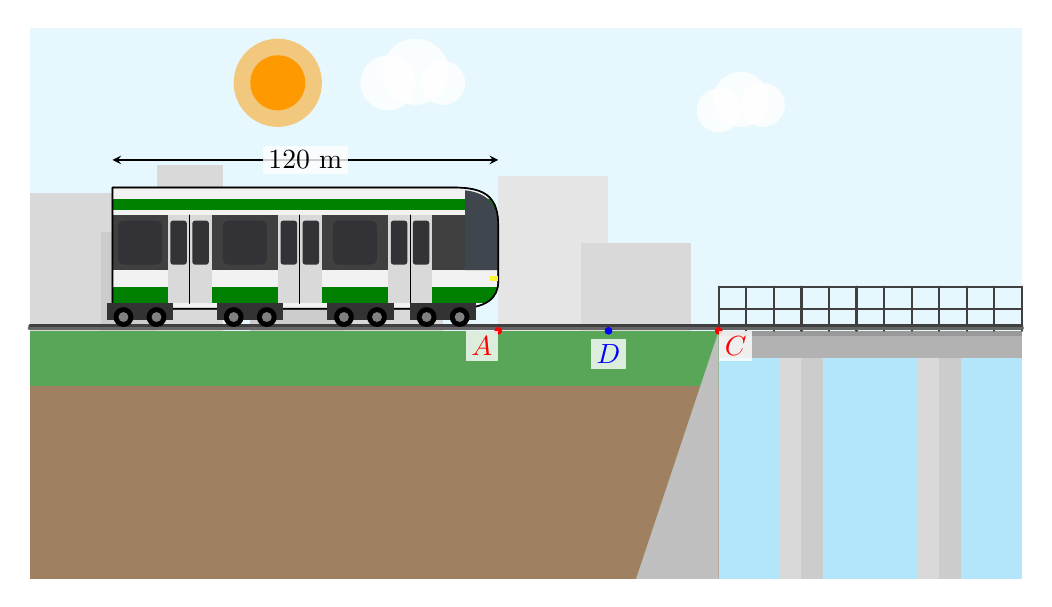
\begin{tikzpicture}[declare function={tL = 4; tLen = 7; tH = 2.2; tY = 0.4; nR = 0.8; wR = 0.18; wY = 0.25; xC = 8;},line join=round,line cap=round,>=stealth,scale=0.7]		
			\fill[cyan!10] (-4.5,0) rectangle (13.5,5.5);
			\fill[gray!30] (-4.5,0) rectangle (-3,2.5);
			\fill[gray!40] (-3.2,0) rectangle (-2,1.8);
			\fill[gray!30] (-2.2,0) rectangle (-1,3.0);
			\fill[gray!40] (-0.5,0) rectangle (1.5,2.2);
			\fill[gray!30] (1.2,0) rectangle (3,1.5);
			\fill[gray!20] (4,0) rectangle (6,2.8);
			\fill[gray!30] (5.5,0) rectangle (7.5,1.6);
			\fill[white,opacity=0.8] (2,4.5) circle (0.5);
			\fill[white,opacity=0.8] (2.5,4.7) circle (0.6);
			\fill[white,opacity=0.8] (3,4.5) circle (0.4);
			\fill[white,opacity=0.8] (8,4.0) circle (0.4);
			\fill[white,opacity=0.8] (8.4,4.2) circle (0.5);
			\fill[white,opacity=0.8] (8.8,4.1) circle (0.4);
			\fill[orange!80!yellow,opacity=0.5] (0,4.5) circle (0.8);
			\fill[orange!80!yellow] (0,4.5) circle (0.5);
			\fill[cyan!30] (xC,-4.5) rectangle (13.5,0);
			\fill[green!30!gray] (-4.5,-1) rectangle (xC,0);
			\fill[brown!50!gray] (-4.5,-4.5) rectangle (xC,-1);
			\fill[gray!50] (xC,-4.5) -- (xC,0) -- (xC-1.5,-4.5) -- cycle;
			\fill[gray!60] (xC,-0.5) rectangle (13.5,0);
			\fill[gray!80] (xC,-0.1) rectangle (13.5,0);
			\foreach \px in {9.5,12.0}{
				\fill[gray!40] (\px-0.4,-4.5) rectangle (\px+0.4,-0.5);
				\fill[gray!30] (\px-0.4,-4.5) rectangle (\px,-0.5);
			}
			
			\draw[line width=0.8pt,gray!50!black] (xC,0.4) -- (13.5,0.4);
			\draw[line width=0.8pt,gray!50!black] (xC,0.8) -- (13.5,0.8);
			\foreach \px in {8.0,8.5,9.0,9.5,10.0,10.5,11.0,11.5,12.0,12.5,13.0,13.5}{
				\draw[line width=0.8pt,gray!50!black] (\px,0) -- (\px,0.8);
			}
			\draw[line width=1.5pt,gray!80!black] (-4.5,0.05) -- (13.5,0.05);
			\draw[line width=1.0pt,gray!50!black] (-4.5,0.1) -- (13.5,0.1);
			\draw[fill=gray!10] (tL-tLen,tY) -- (tL-nR,tY).. controls (tL-0.2,tY) and (tL,tY+0.2).. (tL,tY+0.5) -- (tL,tY+1.5).. controls (tL,tY+tH-0.2) and (tL-0.2,tY+tH).. (tL-nR,tY+tH) -- (tL-tLen,tY+tH) -- cycle;
			
			\begin{scope}
				\clip (tL-tLen,tY) -- (tL-nR,tY).. controls (tL-0.2,tY) and (tL,tY+0.2).. (tL,tY+0.5) -- (tL,tY+1.5).. controls (tL,tY+tH-0.2) and (tL-0.2,tY+tH).. (tL-nR,tY+tH) -- (tL-tLen,tY+tH) -- cycle;
				\fill[green!50!black] (tL-tLen,tY+0.1) rectangle (tL,tY+0.4);
				\fill[darkgray] (tL-tLen,tY+0.7) rectangle (tL,tY+1.7);
				\fill[green!50!black] (tL-tLen,tY+1.8) rectangle (tL,tY+2.0);
				\fill[cyan!20!black] (tL,tY+0.7) -- (tL,tY+1.5).. controls (tL,tY+1.9) and (tL-0.2,tY+2.1).. (tL-0.6,tY+2.15) -- (tL-0.6,tY+0.7) -- cycle;
				
				\foreach \dx in {1.0,3.0,5.0}{
					\fill[gray!30] (tL-tLen+\dx,tY+0.1) rectangle (tL-tLen+\dx+0.8,tY+1.7);
					\draw[line width=0.4pt] (tL-tLen+\dx+0.4,tY+0.1) -- (tL-tLen+\dx+0.4,tY+1.7);
					\fill[cyan!10!black,rounded corners=1pt] (tL-tLen+\dx+0.05,tY+0.8) rectangle (tL-tLen+\dx+0.35,tY+1.6);
					\fill[cyan!10!black,rounded corners=1pt] (tL-tLen+\dx+0.45,tY+0.8) rectangle (tL-tLen+\dx+0.75,tY+1.6); }
				\foreach \dx in {0.1,2.0,4.0}{
					\fill[cyan!10!black,rounded corners=2pt] (tL-tLen+\dx,tY+0.8) rectangle (tL-tLen+\dx+0.8,tY+1.6); }
			\end{scope}
			
			\draw[line width=0.6pt] (tL-tLen,tY) -- (tL-nR,tY).. controls (tL-0.2,tY) and (tL,tY+0.2).. (tL,tY+0.5) -- (tL,tY+1.5).. controls (tL,tY+tH-0.2) and (tL-0.2,tY+tH).. (tL-nR,tY+tH) -- (tL-tLen,tY+tH) -- cycle;
			\fill[yellow!80!white] (tL-0.15,tY+0.5) rectangle (tL,tY+0.6);
			\foreach \dx in {0.5,2.5,4.5,6.0}{
				\fill[black!80] (tL-tLen+\dx-0.6,tY-0.2) rectangle (tL-tLen+\dx+0.6,tY+0.1);
				\fill[black] (tL-tLen+\dx-0.3,wY) circle (wR);
				\fill[black] (tL-tLen+\dx+0.3,wY) circle (wR);
				\fill[gray] (tL-tLen+\dx-0.3,wY) circle (wR/2);
				\fill[gray] (tL-tLen+\dx+0.3,wY) circle (wR/2);
			}
			\draw[<->] (tL-tLen,tY+tH+0.5) -- (tL,tY+tH+0.5) node[midway,fill=white,fill opacity=0.8,text opacity=1,inner sep=2pt] {$120$ m};
			\fill[red] (tL,0) circle (2pt) node[below left,fill=white,fill opacity=0.8,text opacity=1,inner sep=2pt] {$A$};
			\fill[red] (xC,0) circle (2pt) node[below right,fill=white,fill opacity=0.8,text opacity=1,inner sep=2pt] {$C$};
			\fill[blue] (6.0,0) circle (2pt) node[below,fill=white,fill opacity=0.8,text opacity=1,inner sep=2pt,shift={(0,-0.1)}] {$D$};
		\end{tikzpicture}
	\end{center}
	\choiceTF
	{\True Tại thời điểm bắt đầu giảm tốc đầu tàu cách $C$ một đoạn bằng $510$ m}
	{$b=2$}
	{$DC=369$ m \textit{(tính theo mét và làm tròn kết quả đến hàng đơn vị)}}
	{Tổng thời gian tính từ lúc giảm tốc tới khi tàu đi qua được cầu là $63$ giây \textit{(tính theo giây và làm tròn kết quả đến hàng đơn vị)}}
	\loigiai{
		\begin{itemchoice}
			\itemch Quãng đường tàu đi được trong $3$ giây đầu (trước khi giảm tốc) là $s_1=30\cdot 3=90$ m. \\
			Khoảng cách ban đầu từ đầu tàu $A$ đến $C$ là $600$ m. \\
			Tại thời điểm bắt đầu giảm tốc, đầu tàu cách $C$ một đoạn bằng $600-90=510$ m. 
			\itemch Gọi $v(t)$ là vận tốc của tàu tại thời điểm $t$ giây kể từ lúc bắt đầu giảm tốc. Ta có
			\[v(t) = \displaystyle\int a(t) \mathrm{\,d}t = \displaystyle\int (-bt) \mathrm{\,d}t = -\dfrac{bt^2}{2} + C_1.\]
			Tại $t=0$, vận tốc tàu là $v(0)=30\Rightarrow C_1=30$. Suy ra $v(t)=-\dfrac{bt^2}{2}+30$. \\
			Sau $10$ giây giảm tốc ($t=10$), tàu đạt vận tốc $10$ m/s nên
			\[v(10) = 10 \Leftrightarrow -\dfrac{b \cdot 10^2}{2} + 30 = 10 \Leftrightarrow 50b = 20 \Leftrightarrow b = 0{,}4.\]
			Vậy $b=0{,}4$.			
			\itemch Với $b=0{,}4$, phương trình vận tốc là $v(t)=-0{,}2t^2+30$. \\
			Quãng đường tàu đi được trong $10$ giây giảm tốc (từ lúc bắt đầu giảm tốc đến điểm $D$) là
			\[s_2 = \displaystyle\int\limits_0^{10} v(t) \mathrm{\,d}t = \displaystyle\int\limits_0^{10} (-0{,}2t^2 + 30) \mathrm{\,d}t =\left.\left( -\dfrac{0{,}2t^3}{3}+30t\right)\right|_0^{10}=-\dfrac{200}{3} + 300 = \dfrac{700}{3}\;\text{m}.\]
			Khoảng cách từ điểm $D$ đến đầu cầu $C$ là
			\[DC=510-s_2=510-\dfrac{700}{3}=\dfrac{830}{3} \approx 277 \;\text{m}.\]
			Vậy $DC\approx 277$ m. 
			
			\itemch Để tàu đi qua cầu cho an toàn, đuôi tàu phải ra khỏi cầu. Quãng đường đầu tàu cần đi thêm (kể từ $D$) là
			\[s_3=DC+L_{\text{cầu}}+L_{\text{tàu}}=\dfrac{830}{3} + 240 + 120 = \dfrac{1\,910}{3}\; \text{m}.\]
			Từ $D$, tàu chuyển động đều với vận tốc $v=10$ m/s. Thời gian để tàu đi hết quãng đường $s_3$ là
			\[t_3=\dfrac{s_3}{10}=\dfrac{1\,910}{30}=\dfrac{191}{3} \;\text{s}.\]
			Tổng thời gian tính từ lúc giảm tốc tới khi tàu đi qua được cầu là
			\[t_{\text{tổng}}=10+t_3=10+\dfrac{191}{3}=\dfrac{221}{3} \approx 74\;\text{s}.\]
			Vậy tổng thời gian khoảng $74$ giây. 
		\end{itemchoice}
	}
\end{ex}
\caukq
\begin{ex}%[2D1H5-8]%[TDMZZ16]%[Lê Hồ Quang Minh]
	Cho một phân xưởng sản xuất một loại sản phẩm có tổng chi phí sản xuất mỗi tháng là $C(x) = 800 \cdot \mathrm{e}^{0{,}005x} + 100$ (triệu đồng), trong đó $x$ là số lượng sản phẩm sản xuất mỗi tháng ($x \in \mathbb{N}^*, 20 \le x \le 600$). Mỗi sản phẩm được bán với giá cố định là $15$ triệu đồng. Để mỗi tháng phân xưởng đạt lợi nhuận không dưới $650$ triệu đồng, thì phân xưởng này cần sản xuất và tiêu thụ ít nhất bao nhiêu sản phẩm (với giả thiết sản xuất ra bao nhiêu sản phẩm đều bán hết)?
	\par\shortans[oly]{184}
	\loigiai{
		Hàm doanh thu khi bán hết $x$ sản phẩm là $R(x) = 15x$ (triệu đồng).\\
		Hàm lợi nhuận của phân xưởng mỗi tháng là
		\[L(x) = R(x) - C(x) = 15x - 800 \cdot \mathrm{e}^{0{,}005x} - 100.\]
		Để lợi nhuận không dưới $650$ triệu đồng thì
		\allowdisplaybreaks
		\begin{eqnarray*}
			&&L(x) \geq 650\\
			&\Leftrightarrow& 15x - 800 \cdot \mathrm{e}^{0{,}005x} - 100 \geq 650\\
			&\Leftrightarrow& 15x - 800 \cdot \mathrm{e}^{0{,}005x} - 750 \geq 0.
		\end{eqnarray*}
		Xét $f(x) = 15x - 800 \cdot \mathrm{e}^{0{,}005x} - 750$, với $x \in \left[20;600\right]$.\\
		Ta có
		\[f'(x) = 15 - 800 \cdot 0,005 \cdot \mathrm{e}^{0{,}005x} = 15 - 4\mathrm{e}^{0{,}005x}.\]
		Cho $f'(x) = 0 \Leftrightarrow \mathrm{e}^{0{,}005x} = \dfrac{15}{4} \Leftrightarrow x= 200\ln\left(\dfrac{15}{4}\right) \approx 264,35 = x_0 \Rightarrow f(x_0) \approx 215{,}27$.\\
		Bảng biến thiên cho hàm số $f(x)$ như sau
		\begin{center}
			
\begin{tikzpicture}
				\tkzTabInit[nocadre=false,lgt=1.5,espcl=2.5,deltacl=0.6]
				{$x$/0.7,$f'(x)$/0.7,$f(x)$/1.5}{$20$,$x_0$,$600$}
				\tkzTabLine{,+,0,-,}   
				\tkzTabVar{-/,+/$f(x_0)$,-/}
			\end{tikzpicture}
		\end{center}
		Dựa vào BBT ta thấy $f(x) \leq 215{,}27$ nên phương trình $f(x) = 0 $ có $2$ nghiệm phân biệt.\\
		Sử dụng MTCT ta giải phương trình $f(x)=0 \Leftrightarrow \hoac{&x \approx 183{,48}\\&x\approx 335{,}62.}$\\
		Do đó bất phương trình trình $f(x) \geq 0 \Leftrightarrow 183{,}48 \leq x \leq 335{,}62$.\\
		Vậy cần sản xuất và tiêu thụ ít nhất $184$ sản phẩm thì lợi nhuận đạt được không dưới $650$ triệu đồng.
	}
\end{ex}

\begin{ex}%[Duong Xuan Loi]%[1H8V6-2]
	Cho hình lăng trụ $ABC.A'B'C'$ có $AB=4$, $AC=6$, $\widehat{BAC}=60^\circ$ và chiều dài cạnh bên $AA'=5$. Biết hình chiếu vuông góc của $C$ trên đáy $(A'B'C')$ là trung điểm của cạnh $B'C'$. Hãy xác định số đo góc nhị diện $[C',AB,C]$ theo đơn vị độ (\textit{làm tròn kết quả đến hàng đơn vị}).
	\loigiai{
		\begin{center}
			\begin{tikzpicture}[scale=1, font=\footnotesize, line join=round, line cap=round,>=stealth]
				\path 
				(0,0) coordinate (A')
				(1.5,-1.5) coordinate (B')
				(4,0) coordinate (C')
				($(C')!1/2!(B')$) coordinate (K)
				($(K)+(0,4)$) coordinate (C)
				($(B')+(C)-(C')$) coordinate (B)
				($(A')+(C)-(C')$) coordinate (A)
				($(C')-(C)+(B)$) coordinate (H)
				($(A)!0.6!(B)$) coordinate (I);
				
				\draw (A)--(B)--(C)--(C')--(B')--(A')--cycle (A)--(C) (B)--(B') (C')--(H)--(B) (C')--(I)--(H);
				\draw[dashed] (A')--(C') (C)--(K) (C')--(B);	
				
				\foreach \p/\q in {A/180,B/220,C/90,A'/180,B'/-90,C'/0,K/-90,H/-90,I/135}
				\fill[black] (\p) circle (1.0pt) node[shift={(\q:3mm)}]{$\p$};
			\end{tikzpicture}
		\end{center}
		Gọi $K$ là trung điểm của $B'C'$. Ta có $CK \perp (A'B'C')$.\\
		Kẻ $C'H \perp (ABC)$ tại $H$. Vì $(ABC) \parallel (A'B'C')$ nên $C'H = CK = h$.\\
		Trong $\triangle ABC$, áp dụng định lý côsin ta có:
		\[ BC = \sqrt{AB^2 + AC^2 - 2AB \cdot AC \cdot \cos 60^\circ} = \sqrt{4^2 + 6^2 - 2 \cdot 4 \cdot 6 \cdot \dfrac{1}{2}} = 2\sqrt{7}. \]
		Suy ra $B'C' = BC = 2\sqrt{7} \Rightarrow KC' = \sqrt{7}$.\\
		Xét tam giác $CC'K$ vuông tại $K$: $h = CK = \sqrt{CC'^2 - KC'^2} = \sqrt{5^2 - (\sqrt{7})^2} = 3\sqrt{2}$.\\
		Kẻ $HI \perp AB$ tại $I$, kết hợp với $C'H \perp (ABC) \Rightarrow C'H \perp AB$. Suy ra $AB \perp (C'HI) \Rightarrow AB \perp C'I$.\\
		Vậy góc nhị diện $[C',AB,C]$ chính là góc nhị diện $[C',AB,H]$, có số đo là $\widehat{C'IH} = \varphi$.\\
		Do $CK \parallel C'H$ và $\overrightarrow{CB} = \overrightarrow{C'B'}$ nên tứ giác $CKHC'$ là hình bình hành. 
		Mặt khác, $K$ là trung điểm của $B'C'$ nên suy ra $H$ là điểm đối xứng của $C$ qua $B$. Khi đó $\overrightarrow{CH} = \dfrac{3}{2}\overrightarrow{CB}$.\\
		Suy ra $HI = \mathrm{d}(H, AB) = \dfrac{3}{2} \mathrm{d}(C, AB) = \dfrac{3}{2} \cdot AC \cdot \sin 60^\circ = \dfrac{3}{2} \cdot 6 \cdot \dfrac{\sqrt{3}}{2} = \dfrac{9\sqrt{3}}{2}$.\\
		Xét tam giác $C'HI$ vuông tại $H$, ta có:
		\[ \tan \varphi = \dfrac{C'H}{HI} = \dfrac{3\sqrt{2}}{\dfrac{9\sqrt{3}}{2}} = \dfrac{2\sqrt{6}}{9} \Rightarrow \varphi \approx 28{,}56^\circ. \]
		Vậy số đo góc nhị diện cần tìm xấp xỉ $29^\circ$.
	}
\end{ex}

\begin{ex}%[2H5K1-7]%[TDMZZ16-19-TLN]%[Nguyễn Văn Sang]
	Trong không gian $Oxyz$ có đơn vị dài trên mỗi trục là centimet, có một con châu chấu điện tử ban đầu đang đứng ở gốc toạ độ $O(0;0;0)$ và tiến hành nhảy vô hạn lần theo các quy tắc sau:
	\begin{itemize}
		\item Nhảy liên tiếp theo hướng ba vectơ theo thứ tự $\vec{i} = (1;0;0)$, $\vec{j} = (0;1;0)$, $\vec{k} = (0;0;1)$.
		\item Bước nhảy ban đầu có độ dài bằng $30$ centimet và nhảy theo hướng $\vec{i}$ trước.
		\item Độ dài mỗi bước nhảy sẽ giảm $10\%$ so với độ dài bước nhảy ngay trước đó.
	\end{itemize}
	%--- Bắt đầu vẽ hình minh hoạ đề bài ---%
	\begin{center}
		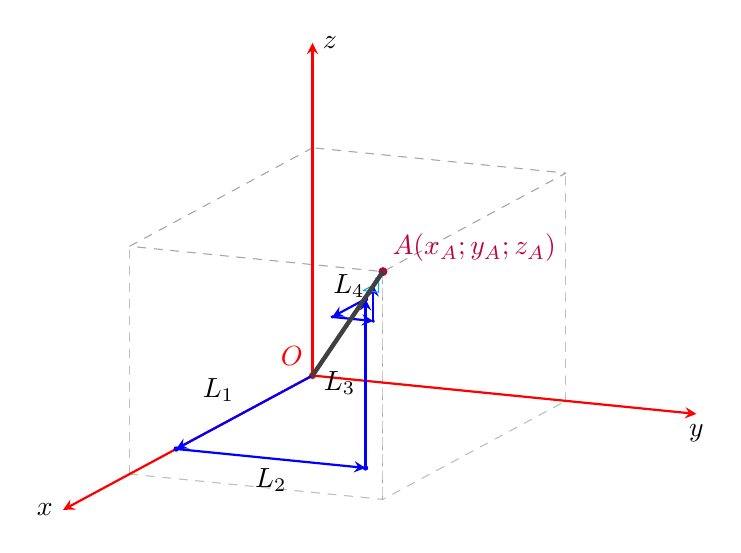
\begin{tikzpicture}[x={(-0.65cm,-0.35cm)}, y={(1cm,-0.1cm)}, z={(0cm,1cm)}, scale=0.65, >=stealth, line join=round, line cap=round]
			% Định nghĩa tọa độ các đỉnh giới hạn của hình hộp chữ nhật O. X-Y-Z
			\coordinate (O) at (0,0,0);
			\coordinate (X) at (5.5,0,0);
			\coordinate (Y) at (0,4.95,0);
			\coordinate (Z) at (0,0,4.45);
			\coordinate (XY) at (5.5,4.95,0);
			\coordinate (XZ) at (5.5,0,4.45);
			\coordinate (YZ) at (0,4.95,4.45);
			\coordinate (XYZ) at (5.5,4.95,4.45); % Vị trí giới hạn của điểm A
			
			% 1. Vẽ các đường nét đứt phía trong của khung hộp 3D trước để không đè lên nét liền
			\draw[dashed, gray!50, thin] (O) -- (X);
			\draw[dashed, gray!50, thin] (O) -- (Y);
			\draw[dashed, gray!50, thin] (O) -- (Z);
			\draw[dashed, gray!50, thin] (X) -- (XY) -- (Y);
			\draw[dashed, gray!50, thin] (X) -- (XZ);
			\draw[dashed, gray!50, thin] (Y) -- (YZ);
			
			% 2. Vẽ các đường nét đứt bao quanh bên ngoài tạo thành khối hộp hoàn chỉnh
			\draw[dashed, gray!70, thin] (Z) -- (XZ) -- (XYZ) -- (YZ) -- cycle;
			\draw[dashed, gray!70, thin] (XY) -- (XYZ);
			
			% Vẽ các đường hạ vuông góc từ điểm giới hạn A xuống các mặt phẳng tọa độ
			\draw[dashed, gray!40] (XYZ) -- (XY);
			
			% 3. Vẽ hệ trục tọa độ Oxyz (Màu đỏ làm điểm nhấn, kéo dài ra ngoài khung hộp)
			\draw[->, red, thick] (O) -- (7.5,0,0) node[left, black] {$x$};
			\draw[->, red, thick] (O) -- (0,7.5,0) node[below, black] {$y$};
			\draw[->, red, thick] (O) -- (0,0,6.5) node[right, black] {$z$};
			\node[above left, red] at (O) {$O$};
			\fill[red] (O) circle (2pt);
			
			% 4. Vẽ các bước nhảy thực tế của con châu chấu (Màu xanh dương đậm, có mũi tên hướng)
			% Bước 1: Dọc theo trục Ox từ O dắt tới P1
			\draw[->, blue, thick] (O) -- (4.1,0,0) node[midway, above left, black] {$L_1$};
			\fill[blue] (4.1,0,0) circle (1.5pt);
			
			% Bước 2: Song song trục Oy từ P1 tới P2
			\draw[->, blue, thick] (4.1,0,0) -- (4.1,3.7,0) node[midway, below, black] {$L_2$};
			\fill[blue] (4.1,3.7,0) circle (1.5pt);
			
			% Bước 3: Song song trục Oz từ P2 tới P3
			\draw[->, blue, thick] (4.1,3.7,0) -- (4.1,3.7,3.3) node[midway, left, black] {$L_3$};
			\fill[blue] (4.1,3.7,3.3) circle (1.5pt);
			
			% Bước 4: Song song trục Ox từ P3 tới P4
			\draw[->, blue, thick] (4.1,3.7,3.3) -- (5.1,3.7,3.3) node[midway, above, black] {$L_4$};
			\fill[blue] (5.1,3.7,3.3) circle (1pt);
			
			% Bước 5: Song song trục Oy từ P4 tới P5
			\draw[->, blue, thick] (5.1,3.7,3.3) -- (5.1,4.5,3.3);
			\fill[blue] (5.1,4.5,3.3) circle (1pt);
			
			% Bước 6: Song song trục Oz từ P5 tới P6
			\draw[->, blue, thick] (5.1,4.5,3.3) -- (5.1,4.5,4.0);
			
			% Đường gấp khúc mờ dần thể hiện xu hướng tiến về vô hạn tại điểm A
			\draw[cyan, thin] (5.1,4.5,4.0) -- (5.4,4.5,4.0) -- (5.4,4.8,4.0) -- (5.4,4.8,4.3) -- (5.5,4.8,4.3);
			
			% 5. Đánh dấu điểm giới hạn A bằng màu tím nổi bật và vẽ đoạn thẳng OA cần tính
			\fill[purple] (XYZ) circle (2.5pt) node[above right, purple] {$A(x_A;y_A;z_A)$};
			\draw[darkgray, ultra thick] (O) -- (XYZ);
		\end{tikzpicture}
	\end{center}
	%--- Kết thúc vẽ hình minh hoạ ---%
	Sau khi nhảy vô hạn lần con châu chấu có vị trí $A$, hãy xác định độ dài đoạn $OA$ theo đơn vị centimet (không làm tròn các phép tính trung gian và làm tròn kết quả cuối cùng đến hàng đơn vị)?
	\par\shortans[0]{174}
	\loigiai{
		Để giải bài toán này một cách dễ hiểu nhất, chúng ta hãy phân tích chuyển động của con châu chấu độc lập trên $3$ trục tọa độ $Ox$, $Oy$, $Oz$. Vì các hướng nhảy $\vec{i}, \vec{j}, \vec{k}$ vuông góc với nhau từng đôi một, tổng quãng đường dịch chuyển trên mỗi hướng chính là tọa độ cuối cùng của điểm $A$.
		\begin{itemize}
			\item Quy luật giảm độ dài: Độ dài bước sau bằng $90\%$ bước trước (giảm $10\%$), tức là nhân với $0{,}9$.
			\item Chu kỳ hướng nhảy: Cứ sau $3$ bước nhảy, con châu chấu lại lặp lại hướng cũ. Do đó, các bước nhảy trên cùng một trục sẽ cách nhau $3$ khoảng, độ dài của chúng sẽ giảm đi một lượng là $0{,}9^3 = 0{,}729$ lần.
		\end{itemize}
		Dưới đây là chi tiết các bước tính toán tọa độ điểm $A(x_A; y_A; z_A)$:
		\begin{enumerate}
			\item \textbf{Tính tọa độ $x_A$ (Các bước nhảy theo hướng trục $Ox$):}
			\begin{itemize}
				\item Con châu chấu nhảy theo trục $Ox$ ở các bước: $1, 4, 7, 10, \dots$
				\item Độ dài tương ứng: $L_1 = 30$, $L_4 = 30 \times 0{,}9^3$, $L_7 = 30 \times 0{,}9^6, \dots$
				\item Đây là một cấp số nhân lùi vô hạn với số hạng đầu $u_1 = 30$ và công bội $q = 0{,}9^3 = 0{,}729$.
				\item Áp dụng công thức tổng cấp số nhân lùi vô hạn $\displaystyle S = \dfrac{u_1}{1-q}$:
				\[ x_A = \displaystyle\dfrac{30}{1 - 0{,}729} = \dfrac{30}{0{,}271} = \dfrac{30000}{271} \text{ (cm)}. \]
			\end{itemize}
			\item \textbf{Tính tọa độ $y_A$ (Các bước nhảy theo hướng trục $Oy$):}
			\begin{itemize}
				\item Con châu chấu nhảy theo trục $Oy$ ở các bước: $2, 5, 8, 11, \dots$
				\item Độ dài tương ứng: $L_2 = 30 \times 0{,}9 = 27$, $L_5 = 27 \times 0{,}9^3$, $L_8 = 27 \times 0{,}9^6, \dots$
				\item Đây là cấp số nhân lùi vô hạn với số hạng đầu $v_1 = 27$ và công bội $q = 0{,}729$.
				\item Tổng tọa độ theo trục $Oy$ là
				\[ y_A = \displaystyle\dfrac{27}{1 - 0{,}729} = \dfrac{27}{0{,}271} = \dfrac{27000}{271} \text{ (cm)}. \]
			\end{itemize}
			\item \textbf{Tính tọa độ $z_A$ (Các bước nhảy theo hướng trục $Oz$):}
			\begin{itemize}
				\item Con châu chấu nhảy theo trục $Oz$ ở các bước: $3, 6, 9, 12, \dots$
				\item Độ dài tương ứng: $L_3 = 30 \times 0{,}9^2 = 24{,}3$, $L_6 = 24{,}3 \times 0{,}9^3$, $L_9 = 24{,}3 \times 0{,}9^6, \dots$
				\item Đây là cấp số nhân lùi vô hạn với số hạng đầu $w_1 = 24{,}3$ và công bội $q = 0{,}729$.
				\item Tổng tọa độ theo trục $Oz$ là
				\[ z_A = \displaystyle\dfrac{24{,}3}{1 - 0{,}729} = \dfrac{24{,}3}{0{,}271} = \dfrac{24300}{271} \text{ (cm)}. \]
			\end{itemize}
			\item \textbf{Tính độ dài đoạn thẳng $OA$:}
			\begin{itemize}
				\item Điểm $A$ chính là đỉnh đối diện của hình hộp chữ nhật có ba kích thước tương ứng là $x_A, y_A, z_A$ tính từ gốc tọa độ $O$.
				\item Khoảng cách $OA$ được tính bằng công thức Pitago trong không gian 3D:
				\begin{align*}
					OA &= \sqrt{x_A^2 + y_A^2 + z_A^2} \\
					&= \sqrt{\left(\dfrac{30000}{271}\right)^2 + \left(\dfrac{27000}{271}\right)^2 + \left(\dfrac{24300}{271}\right)^2} \\
					&\approx 174 \text{ (cm)}.
			\end{align*}\end{itemize}
		\end{enumerate}
		Vậy độ dài đoạn thẳng $OA$ xấp xỉ $174$ centimet.
	}
\end{ex}

\begin{ex}%[1D7C2-8]%[TDMZZ16]%[Nguyễn Đức Tuấn Anh]
	\immini[thm]{
		Cho một bình ban đầu chưa đựng gì như hình vẽ bên dưới, bình có dạng hình lăng trụ đều với cạnh đáy bằng $60$ cm và cạnh bên bằng $90$ cm bên trong có một quả cầu đặc bán kính $20$ cm không thấm nước. Ở thời điểm ban đầu $t_0=0$ ta tiến hành dùng một vòi nước cho chảy vào bình với lưu lượng không đổi bằng $L$ cm$^3$/phút. Biết rằng sau khoảng thời gian $120$ phút thì vòi chảy đầy bình. Hãy tính theo đơn vị cm/phút tốc độ dâng của mực nước trong bình ở thời điểm $15$ phút (\textit{không làm tròn ở các phép tính trung gian và làm tròn kết quả cuối cùng đến hàng phần mười}).}{
		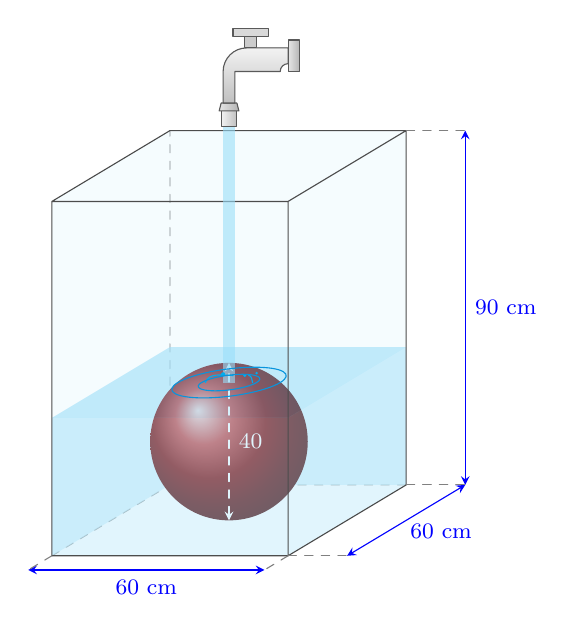
\begin{tikzpicture}[line cap=round, line join=round, >=stealth,3dview/.style={x={(1cm,0cm)}, y={(0.5cm,0.3cm)}, z={(0cm,1cm)}},3dview, scale=0.5,font=\footnotesize]
			\foreach \x/\y/\n in {0/0/A, 6/0/B, 6/6/C, 0/6/D} {
				\coordinate (\n) at (\x,\y,0);
				\coordinate (\n') at (\x,\y,9);
				\coordinate (W\n) at (\x,\y,3.5);
			}
			\coordinate (O) at (3,3,2);
			
			\draw[dashed, gray!80] (A) -- (D) -- (C) (D) -- (D');
			
			\fill[cyan!10, opacity=0.4] (A)--(D)--(D')--(A')--cycle (D)--(C)--(C')--(D')--cycle;
			\fill[cyan!30, opacity=0.4] (A)--(D)--(WD)--(WA)--cycle (D)--(C)--(WC)--(WD)--cycle;
			
			\begin{scope}[shift={(O)}, x={(1cm,0cm)}, y={(0cm,1cm)}]
				\shade[ball color=red!70!black] (0,0) circle (2);
				\draw[white, stealth-stealth, dashed] (0,-2) -- (0,2) node[midway, right] {40};
			\end{scope}
			
			\fill[cyan!40, opacity=0.4] (WA)--(WB)--(WC)--(WD)--cycle;
			\fill[cyan!30, opacity=0.4] (A)--(B)--(WB)--(WA)--cycle (B)--(C)--(WC)--(WB)--cycle;
			
			\draw[black!70] (A) -- (B) -- (C) (A) -- (A') (B) -- (B') (C) -- (C') (A') -- (B') -- (C') -- (D') -- cycle;
			
			\fill[cyan!40, opacity=0.6] (2.85, 3, 3.5) -- (3.15, 3, 3.5) -- (3.15, 3, 10.3) -- (2.85, 3, 10.3) -- cycle;
			
			\begin{scope}[shift={(3,3,3.5)}, x={(1cm,0cm)}, y={(0.5cm,0.3cm)}]
				\draw[cyan] (-0.6,0) to[out=70, in=180] (-0.2,0.6);
				\draw[cyan] (0.6,0) to[out=110, in=0] (0.2,0.6);
				\fill[cyan] (-0.5,0.7) circle (1.5pt);
				\fill[cyan] (0.3,0.8) circle (1pt);
				\fill[cyan] (0.1,0.6) circle (1.2pt);
				\draw[cyan!80!blue, thin] (0,0) ellipse (1.3 and 1.3);
				\draw[cyan!80!blue, thin] (0,0) ellipse (0.7 and 0.7);
			\end{scope}
			
			\begin{scope}[shift={(3,3,10)}, x={(1cm,0cm)}, y={(0cm,1cm)}]
				\filldraw[left color=gray!10, right color=gray!50, draw=gray!70!black] (-0.2,0) rectangle (0.2, 0.4);
				\filldraw[left color=gray!20, right color=gray!60, draw=gray!70!black] (-0.25, 0.4) -- (0.25, 0.4) -- (0.2, 0.6) -- (-0.2, 0.6) -- cycle;
				\filldraw[top color=gray!10, bottom color=gray!50, draw=gray!70!black] (-0.15, 0.6) -- (-0.15, 1.4) arc(180:90:0.6) -- (1.5, 2.0) -- (1.5, 1.6) arc(90:180:0.2) -- (0.15, 1.4) -- (0.15, 0.6) -- cycle;
				\filldraw[left color=gray!20, right color=gray!60, draw=gray!70!black] (1.5, 1.4) rectangle (1.8, 2.2);
				\filldraw[fill=gray!40, draw=gray!70!black] (0.4, 2.0) rectangle (0.7, 2.3);
				\filldraw[fill=gray!30, draw=gray!70!black] (0.1, 2.3) rectangle (1.0, 2.5);
			\end{scope}
			
			\draw[stealth-stealth, blue] (0,-1.2,0) -- (6,-1.2,0) node[midway, below] {60 cm};
			\draw[dashed, gray] (A) -- (0,-1.2,0) (B) -- (6,-1.2,0);
			
			\draw[stealth-stealth, blue] (7.5,0,0) -- (7.5,6,0) node[midway, below right=-2pt] {60 cm};
			\draw[dashed, gray] (B) -- (7.5,0,0) (C) -- (7.5,6,0);
			
			\draw[stealth-stealth, blue] (7.5,6,0) -- (7.5,6,9) node[midway, right] {90 cm};
			\draw[dashed, gray] (C) -- (7.5,6,0) (C') -- (7.5,6,9);
			
		\end{tikzpicture}
	}
	\par\shortans{1{,}0}
	\loigiai{
		Thể tích của toàn bộ bình là $V_{\text{bình}} = 60^2 \cdot 90 = 324\,000\,\left(\text{cm}^3\right)$.\\
		Thể tích của quả cầu là $V_{\text{cầu}} = \dfrac{4}{3}\pi \cdot 20^3 = \dfrac{32\,000\pi}{3}\,\left(\text{cm}^3\right)$.\\
		Thể tích nước cần để chảy đầy bình là $V = V_{\text{bình}} - V_{\text{cầu}} = 324\,000 - \dfrac{32\,000\pi}{3}\,\left(\text{cm}^3\right)$.\\
		Lưu lượng nước chảy vào bình là $L = \dfrac{V}{120} = 2\,700 - \dfrac{800\pi}{9}\,\left(\text{cm}^3/\text{phút}\right)$.\\
		Thời gian để nước ngập hoàn toàn quả cầu (chiều cao mực nước $h = 40$ cm) là
		\[t_2 = \dfrac{60^2 \cdot 40 - V_{\text{cầu}}}{L} \approx 45{,}64 \text{ (phút)}.\]
		Vì $15 < t_2$ nên tại thời điểm $t = 15$ phút, mực nước trong bình có độ cao $h$ thỏa mãn $0 < h < 40$.\\
		Thể tích phần chỏm cầu bị ngập trong nước khi mực nước đạt độ cao $h$ là
		\[V_{\text{chỏm}}(h) = \pi h^2 \left(20 - \dfrac{h}{3}\right).\]
		Thể tích nước trong bình tại thời điểm $t$ tương ứng với chiều cao mực nước $h$ là
		\[V(h) = 60^2 \cdot h - V_{\text{chỏm}}(h) = 3\,600h - \pi h^2 \left(20 - \dfrac{h}{3}\right) = \dfrac{\pi}{3}h^3 - 20\pi h^2 + 3\,600h.\]
		Mặt khác, ta cũng có
		\[V(h) = L \cdot t. \quad (1)\]
		Tại thời điểm $t = 15$ phút, thay vào $(1)$ ta được phương trình
		\[\dfrac{\pi}{3}h^3 - 20\pi h^2 + 3\,600h = 15L.\]
		Giải phương trình này ta thu được nghiệm $h_1 \approx 12{,}137$ (cm).\\
		Đạo hàm hai vế của $(1)$ theo biến $t$ ta được
		\[V'(h) \cdot h'(t) = L \Leftrightarrow (\pi h^2 - 40\pi h + 3\,600) \cdot h'(t) = L.\]
		Suy ra tốc độ dâng của mực nước tại thời điểm $t$ là
		\[h'(t) = \dfrac{L}{\pi h^2 - 40\pi h + 3\,600}.\]
		Thay $h = h_1$ vào biểu thức trên, ta tính được tốc độ dâng của mực nước ở thời điểm $15$ phút là
		\[h'(15) = \dfrac{L}{\pi h_1^2 - 40\pi h_1 + 3\,600} \approx 1{,}0 \text{ (cm/phút)}.\]
	}
\end{ex}

\begin{ex}%[2H5C3-4]%[TDMZZ16]%[Trương Tường]
	Trong không gian $Oxyz$ có đơn vị dài trên mỗi trục là mét, có hai vật $X$ và $Y$ tham gia hai chuyển động trên hai quỹ đạo. Vật $X$ luôn cách gốc toạ độ $O$ và điểm $A(40;30;0)$ những khoảng lần lượt là $40 \, \text{m}$ và $30 \, \text{m}$, vật $Y$ chuyển động trên đường thẳng 
	$d \colon \heva{&x=60+3t \\ &y=50-4t \\ &z=20+t}$. Hãy xác định khoảng cách ngắn nhất có thể giữa hai vật $X$ và $Y$ theo đơn vị centimet (không làm tròn các phép tính trung gian và làm tròn kết quả cuối cùng đến hàng đơn vị)?
	\par\shortans[oly]{$4600$}
	\loigiai{
		\begin{center}
			\begin{tikzpicture}[scale=0.6, >=stealth, line join=round, line cap=round, font=\footnotesize]
				\def\a{3}
				\def\b{1}
				\def\g{20} % góc quay
				\def\G{20} % góc xác định tiếp điểm
				\def\GA{-15} % góc xác định tiếp điểm
				\pgfmathsetmacro{\ux}{-\a*sin(\G)*cos(\g)-\b*cos(\G)*sin(\g)}
				\pgfmathsetmacro{\uy}{-\a*sin(\G)*sin(\g)+\b*cos(\G)*cos(\g)}
				%
				\pgfmathsetmacro{\uxa}{-\a*sin(\GA)*cos(\g)-\b*cos(\GA)*sin(\g)}
				\pgfmathsetmacro{\uya}{-\a*sin(\GA)*sin(\g)+\b*cos(\GA)*cos(\g)}
				%
				\path (0,0) coordinate (I)
				\foreach \l/\ang in {A1/0, A2/180, B1/90, B2/270, M/{\G}, X/-60, N/{\GA}}{
					({\a*cos(\ang)*cos(\g)-\b*sin(\ang)*sin(\g)},{\a*cos(\ang)*sin(\g)+\b*sin(\ang)*cos(\g)}) coordinate (\l)
				}
				(M)+(\ux,\uy) coordinate (M1)
				($(M)!1!90:(M1)$) coordinate (M')
				(intersection of B1--B2 and M--M') coordinate (O)
				(N)+(\uxa,\uya) coordinate (N1)
				($(N)!1!-90:(N1)$) coordinate (N')
				(intersection of B1--B2 and N--N') coordinate (A)
				($(A)!.5!(O)$) coordinate (J)
				;
				\draw [samples=100, smooth, dash pattern=on 1.5pt off 1.5pt] plot [domain={\GA}:{180-\GA}] ({\a*cos(\x)*cos(\g)-\b*sin(\x)*sin(\g)},{\a*cos(\x)*sin(\g)+\b*sin(\x)*cos(\g)})
				;
				\fill [samples=100, smooth, pattern=dots] plot [domain={0}:{360}] ({\a*cos(\x)*cos(\g)-\b*sin(\x)*sin(\g)},{\a*cos(\x)*sin(\g)+\b*sin(\x)*cos(\g)})
				;
				\path (I)--(A2) node [pos=.5, fill=white, inner sep=.5pt] {$(P)$};
				\draw [dash pattern=on 1.5pt off 1.5pt] (O)--(A)--(X) node [above, pos=.5, sloped] {$30$}--cycle node [below, pos=.5, sloped] {$40$};
				\draw [black, ball color=cyan, opacity=.5]
				(O) let \p1=($(M)-(O)$) in circle ({veclen(\p1)});
				\draw [blue, ball color=red, opacity=.5]
				(A) let \p1=($(N)-(A)$) in circle ({veclen(\p1)})
				;
				\draw [samples=100, smooth] plot [domain={-\GA-180}:{\GA}] ({\a*cos(\x)*cos(\g)-\b*sin(\x)*sin(\g)},{\a*cos(\x)*sin(\g)+\b*sin(\x)*cos(\g)});
				\foreach \x/\y in {X/80, O/-90, A/90, I/180}{
					\draw [fill=black] (\x) circle (1pt) ++(\y:0.4) node {$\x$};
				}
			\end{tikzpicture}
		\end{center}
		Do vật $X$ luôn cách gốc tọa độ $O$ một khoảng $R_1=40$ và cách điểm $A(40;30;0)$ một khoảng $R_2=30$ nên $X$ luôn nằm trên đường tròn giao tuyến $(\mathcal{C})$ của hai mặt cầu sau
		\begin{itemize}
			\item Mặt cầu $(S_1)$ tâm $O$, bán kính $R_1=40$ có phương trình $x^2+y^2+z^2=1\,600 \quad (1)$.
			\item Mặt cầu $(S_2)$ tâm $A$, bán kính $R_2=30$ có phương trình 
			\[(x-40)^2+(y-30)^2+z^2=900 \Leftrightarrow x^2+y^2+z^2-80x-60y=-1\,600 \quad (2).\]
		\end{itemize}
		Lấy $(1)$ trừ $(2)$ theo vế ta có 
		\[80x+60y=3\,200 \Leftrightarrow 4x+3y-160=0.\]
		Đây là phương trình mặt phẳng $(P)$ chứa đường tròn $(\mathcal{C})$. \\
		Mặt phẳng $(P)$ có vectơ pháp tuyến $\overrightarrow{n}=(4;3;0)$. \\
		Đường thẳng $d$ đi qua điểm $D(60;50;20)$ và có vectơ chỉ phương $\overrightarrow{u}=(3;-4;1)$. \\
		Lại có
		\[\overrightarrow{u} \cdot \overrightarrow{n}=4 \cdot 3+3 \cdot (-4)+0 \cdot 1=0.\]
		Suy ra $\overrightarrow{u} \perp \overrightarrow{n}$. \\
		Mà $M \notin (P)$ nên $d \parallel (P)$. 
		\begin{center}
			\begin{tikzpicture}[scale=0.6, >=stealth, line join=round, line cap=round, font=\footnotesize]
				\def\a{3}
				\def\b{1}
				\path (0,0) coordinate (I)
				(I)+(1.25*\a,-1.8*\b) coordinate (P1)
				++(2*\a,1.8*\b) coordinate (P2)
				(I)++(-1.25*\a,1.8*\b) coordinate (P3)
				++($(P1)-(P2)$) coordinate (P4)
				($({\a*cos(110)},{\b*sin(110)})+(I)$) coordinate (a1) coordinate (N)
				($({\a*cos(-150)},{\b*sin(-150)})+(I)$) coordinate (a2) coordinate (M)
				(a1)++(90:4) coordinate (d1)
				(a2)++(90:4) coordinate (d2)
				($(a1)!.5!(a2)$) coordinate (Y') 
				++(90:4) coordinate (Y)
				($({\a*cos(30)},{\b*sin(30)})+(I)$) coordinate (X)
				($(d1)!-.15!(d2)$) coordinate (D)
				;
				\pic [draw, "$P$", angle radius=0.3cm, angle eccentricity=.5] {angle=P2--P1--P4};
				\pic [draw, angle radius=0.15cm] {right angle=M--Y'--I};
				\pic [draw, angle radius=0.15cm] {right angle=X--Y'--Y};
				\pic [draw, angle radius=0.15cm] {right angle=Y--Y'--a1};
				\draw (P1)--(P2)--(P3)--(P4)--cycle;
				\draw [semithick] (I) ellipse ({\a} and {\b})
				($(a1)!-.5!(a2)$)--($(a2)!-.65!(a1)$) node [left] {$d'$}
				($(d1)!-.5!(d2)$)--($(d2)!-.65!(d1)$) node [left] {$d$}
				(X)--(Y)--(Y') node [below, pos=.5, sloped] {$46$}--cycle
				(I)--(Y') node [below, pos=.5] {$d$}
				;
				\foreach \x/\y in {I/-90, Y/90, Y'/180, X/80, M/-90, N/90, D/90}{
					\draw [fill=black] (\x) circle (1pt) ++(\y:0.4) node {$\x$};
				}
			\end{tikzpicture}
			\hspace*{.5cm}
			\begin{tikzpicture}[scale=0.6, >=stealth, line join=round, line cap=round, font=\footnotesize]
				\def\a{3}
				\def\b{1}
				\path (0,0) coordinate (I)
				(I)+(1.25*\a,-1.8*\b) coordinate (P1)
				++(2*\a,1.8*\b) coordinate (P2)
				(I)++(-1.25*\a,1.8*\b) coordinate (P3)
				++($(P1)-(P2)$) coordinate (P4)
				($({\a*cos(110)},{\b*sin(110)})+(I)$) coordinate (a1)
				($({\a*cos(-150)},{\b*sin(-150)})+(I)$) coordinate (a2) coordinate (X)
				(a1)++(90:4) coordinate (d1)
				(a2)++(90:4) coordinate (d2)
				(X)++(90:4) coordinate (Y)
				;
				\pic [draw, "$P$", angle radius=0.3cm, angle eccentricity=.5] {angle=P2--P1--P4};
				\pic [draw, angle radius=0.15cm] {right angle=N--X--Y};
				\pic [draw, angle radius=0.15cm] {right angle=d1--Y--X};
				\draw (P1)--(P2)--(P3)--(P4)--cycle;
				\draw [semithick] (I) ellipse ({\a} and {\b})
				($(a1)!-.5!(a2)$)--($(a2)!-.65!(a1)$) node [left] {$d'$}
				($(d1)!-.5!(d2)$)--($(d2)!-.65!(d1)$) node [left] {$d$}
				(Y)--(X) node [below, pos=.5, sloped, rotate=180] {$46$}
				;
				\foreach \x/\y in {I/-90, Y/90, X/-90, N/90}{
					\draw [fill=black] (\x) circle (1pt) ++(\y:0.4) node {$\x$};
				}
			\end{tikzpicture}
		\end{center}
		Gọi $I$ là tâm của đường tròn $(\mathcal{C})$, khi đó $I$ là hình chiếu của $O$ trên $(P)$. \\
		Mặt cầu $(S_1)$ có bán kính $R_1=40$. \\
		Khoảng cách $d$ từ $O$ đến $(P)$ là $d=\dfrac{|4 \cdot 0+3 \cdot 0-160|}{\sqrt{4^2+3^2+0^2}}=32$. \\
		Bán kính của $(\mathcal{C})$ là $r=\sqrt{R_1^2-d^2}=\sqrt{40^2-32^2}=24$. \\
		Ta có $\overrightarrow{OA}=(40;30;0)$. \\
		Chọn $\overrightarrow{u'}=\dfrac{1}{10} \cdot \overrightarrow{OA}=(4;3;0)$ là vectơ chỉ phương của đường thẳng $OA$. \\
		Phương trình đường thẳng $OA$ là $\heva{&x=4t' \\ &y=3t' \\ &z=0.}$ \\
		Vì $I$ là giao điểm của đường thẳng $OA$ và mặt phẳng $(P)$ nên tọa độ điểm $I$ thỏa mãn hệ phương trình 
		\[\heva{&x=4t' \\ &y=3t' \\ &z=0 \\ &4x+3y-160=0} \Leftrightarrow \heva{&t'=6{,}4 \\ &x=25{,}6 \\ &y=19{,}2 \\ &z=0.}\]
		Do đó $I(25{,}6;19{,}2;0)$. \\
		Gọi $d'$ là hình chiếu của $d$ trên $(P)$, $Y'$ là hình chiếu của $Y$ trên $(P)$. \\
		Vì $d \parallel (P)$ nên 
		\[YY'=d(Y,(P))=d(M,(P))=\dfrac{|4 \cdot (60+3t)+3 \cdot (50-4t)-160|}{\sqrt{4^2+3^2+0^2}}=\frac{230}{5}=46.\]
		Gọi $(Q)$ là mặt phẳng chứa $d$ và $d'$. Khi đó $(Q)$ có cặp vectơ chỉ phương là $\overrightarrow{u}$ và $\overrightarrow{n}$. \\
		Chọn $\overrightarrow{n'}=\left[\overrightarrow{u},\overrightarrow{n}\right]=(-3;4;25)$ là vectơ pháp tuyến của $(Q)$. \\
		Mặt phẳng $(Q)$ đi qua điểm $D$ và có vectơ pháp tuyến $\overrightarrow{n'}$ nên có phương trình 
		\[-3(x-60)+4(y-50)+25(z-20)=0 \Leftrightarrow -3x+4y-25z+520=0.\]
		Ta có 
		\[d(I,d')=d(I,(Q))=\dfrac{|-3 \cdot 25{,}6+4 \cdot 19{,}2-25 \cdot 0+520|}{\sqrt{(-3)^2+4^2+25^2}}=4\sqrt{26}<r.\]
		Do đó $d'$ cắt $(\mathcal{C})$ tại hai điểm phân biệt $M$, $N$. \\
		Với ba điểm $X$, $Y$, $Y'$ ta có $XY \ge YY'=46$. \\
		Do đó $XY$ nhỏ nhất bằng $46$ khi $X$ trùng $M$ hoặc $X$ trùng $N$. \\
		Vậy khoảng cách ngắn nhất của hai vật $X$ và $Y$ là $46$ m $=4\,600$ cm.
	}
\end{ex}

\begin{ex}%[2D6C1-2]
	Xếp ngẫu nhiên ba học sinh lớp A, ba học sinh lớp B, hai học sinh lớp C vào 5 phòng học. Gọi $p$ là xác suất để sao cho không có hai học sinh cùng lớp cùng phòng, nếu đã biết mỗi phòng có ít nhất một học sinh. Hãy tính $10^4 p$ (không làm tròn ở các phép tính trung gian và làm tròn kết quả cuối cùng đến hàng đơn vị).
	\par
	\shortans{3143}
	\loigiai{
		Tổng số học sinh là $3+3+2 = 8$ học sinh.\\
		Gọi $X$ là biến cố \lq\lq không có hai học sinh cùng lớp cùng phòng\rq\rq.\\
		$Y$ là biến cố \lq\lq mỗi phòng có ít nhất một học sinh\rq\rq.\\
		Ta cần tính $p=\mathrm{P}\left(X\mid Y\right)=\dfrac{n(XY)}{n(Y)}$.
		\begin{itemize}
			\item $n(Y)$ là số cách xếp $8$ người vào $5$ phòng sao cho mỗi phòng có ít nhất $1$ người. Có các khả năng về số người trong mỗi phòng là $(1,1,1,1,4)$, $(1,1,1,2,3)$, $(1,1,2,2,2)$.\\
			Ta có $n(Y)=\dfrac{5!}{4!}\cdot \dfrac{8!}{4!}+\dfrac{5!}{3!}\cdot \dfrac{8!}{2!3!}+\dfrac{5!}{2!3!}\cdot \dfrac{8!}{2!2!2!}=126\,000$.
			\item $n(X)$ là số cách xếp sao cho không có hai học sinh cùng lớp cùng phòng.\\
			Ta có $n(X)=\mathrm{A}^3_5\cdot \mathrm{A}^3_5\cdot \mathrm{A}^2_5$.\\
			$n(X\overline{Y})$ là số cách xếp sao cho không có hai học sinh cùng lớp cùng phòng và có phòng không có học sinh nào (suy ra có tối đa $2$ phòng trống). Do đó
			$$n(X\overline{Y})=\mathrm{C}^1_5\cdot\mathrm{A}^3_4\cdot \mathrm{A}^3_4\cdot \mathrm{A}^2_4-\mathrm{C}^2_5\cdot\mathrm{A}^3_3\cdot \mathrm{A}^3_3\cdot \mathrm{A}^2_3.$$
			Từ đó ta có
			$$n(XY)=n(X)-n(X\overline{Y})=\mathrm{A}^3_5\cdot \mathrm{A}^3_5\cdot \mathrm{A}^2_5-\mathrm{C}^1_5\cdot\mathrm{A}^3_4\cdot \mathrm{A}^3_4\cdot \mathrm{A}^2_4+\mathrm{C}^2_5\cdot\mathrm{A}^3_3\cdot \mathrm{A}^3_3\cdot \mathrm{A}^2_3=39\,600.$$
		\end{itemize}
		Vậy $p=\mathrm{P}\left(X\mid Y\right)=\dfrac{n(XY)}{n(Y)}=\dfrac{39\,600}{126\,000}=\dfrac{11}{35}$.\\
		Bởi vậy $10^4p=10^4\cdot \dfrac{11}{35}\approx 3143$.
	}
\end{ex}

